\PassOptionsToPackage{xetex}{xcolor}
\PassOptionsToPackage{xetex}{graphicx}
\documentclass[a4paper,landscape,headrule,footrule,xetex]{foils}

%%
%%%  Macros
%%%
\newcommand{\logo}{~}
\MyLogo{HG8011 (2019)}
\newcommand{\Story}{\SHA{HOUN}{The Hound of the Baskervilles}}

\newcommand{\header}[3]{%
\title{\vspace*{-2ex} \large Detecting Meaning with Sherlock Holmes\thanks{Creative Commons Attribution License: you are free to share and adapt as long as you give appropriate credit and add no additional restrictions: 
\protect\url{https://creativecommons.org/licenses/by/4.0/}.}
%\footnotemark
\\[2ex] \Large  \emp{#2} \\ \emp{#3}}
\author{\blu{Francis Bond}   \\ 
\normalsize  \textbf{Division of Linguistics and Multilingual Studies}\\
\normalsize  \url{http://www3.ntu.edu.sg/home/fcbond/}\\
\normalsize  \texttt{bond@ieee.org}}
 \date{Location: LT25}
 \renewcommand{\logo}{#2}
 \hypersetup{
   pdfinfo={
     Author={Francis Bond},
     Title={#2},
     Subject={HG8011: Detecting Meaning with Sherlock Holmes},
     Keywords={Semantics, Pragmatics, Meaning},
     License={CC BY 4.0}
   }
 %  pdfcopyright={Copyright © Francis Bond. Creative Commons 4.0 Attribution License.}
 %  pdflicenseurl={http://creativecommons.org/licenses/by/4.0/}
 }
}
%%
%% Multilingual Stuff
%%
\usepackage[a4paper,landscape,margin=25mm]{geometry}

\usepackage{fontenc}
\usepackage{polyglossia}
\setmainlanguage{english}
\setmainfont{TeX Gyre Pagella}
\usepackage{xeCJK}
\setCJKmainfont{Noto Sans CJK SC}
\setCJKsansfont{Noto Sans CJK SC}
\setCJKmonofont{Noto Sans CJK SC}
%\setCJKttfont{Noto Sans CJK SC}
%\setCJKmainfont{WenQuanYi Micro Hei}
%\clearpage
%\setCJKmainfont{AR PL SungtiL GB}

\usepackage[xetex]{xcolor}
\usepackage[xetex]{graphicx}
\newcommand{\blu}[1]{\textcolor{blue}{#1}}
\newcommand{\grn}[1]{\textcolor{green}{#1}}
\newcommand{\hide}[1]{\textcolor{white}{#1}}
\newcommand{\emp}[1]{\textcolor{red}{#1}}
\newcommand{\txx}[1]{\textbf{\textcolor{blue}{#1}}}
\newcommand{\lex}[1]{\textbf{\mtcitestyle{#1}}}

\usepackage{pifont}
\renewcommand{\labelitemi}{\textcolor{violet}{\ding{227}}}
\renewcommand{\labelitemii}{\textcolor{purple}{\ding{226}}}

\newcommand{\subhead}[1]{\noindent\textbf{#1}\\[5mm]}

\newcommand{\Bad}{\emp{\raisebox{0.15ex}{\ensuremath{\mathbf{\otimes}}}}}
\newcommand{\bad}{*}

\newcommand{\com}[1]{\hfill \textnormal{(\emp{#1})}}%
\newcommand{\cxm}[1]{\hfill \textnormal{(\txx{#1})}}%
\newcommand{\cmm}[1]{\hfill \textnormal{(#1)}}%
\usepackage{amssymb}
\usepackage{relsize,xspace}
\newcommand{\into}{\ensuremath{\rightarrow}\xspace}
\newcommand{\ent}{\ensuremath{\Rightarrow}\xspace}
\newcommand{\nent}{\ensuremath{\not\Rightarrow}\xspace}
\newcommand{\tot}{\ensuremath{\leftrightarrow}\xspace}
\usepackage{url}
\usepackage[hidelinks]{hyperref}
\hypersetup{
     colorlinks,
     linkcolor={blue!50!black},
     citecolor={red!50!black},
     urlcolor={blue!80!black}
}
%\usepackage{hyperxmp}
\newcommand{\lurl}[1]{\MyLogo{\url{#1}}}

\usepackage{mygb4e}
\let\eachwordone=\itshape
\newcommand{\lx}[1]{\textbf{\textit{#1}}}
\newcommand{\ix}{\ex\it}

\newcommand{\cen}[2]{\multicolumn{#1}{c}{#2}}
%\usepackage{times}
%\usepackage{nttfoilhead}
\newcommand{\myslide}[1]{%
\foilhead[-25mm]{\raisebox{12mm}[0mm]{\emp{#1}}}%
\leftheader{}%
\MyLogo{\logo}}

\newcommand{\mytask}[1]{%
\foilhead[-25mm]{\raisebox{12mm}[0mm]{\emp{#1}}}
\leftheader{🔍 Hi}%
\MyLogo{\logo}}

\newcommand{\myslider}[1]{\rotatefoilhead[-25mm]{\raisebox{12mm}[0mm]{\emp{#1}}}}
%\newcommand{\myslider}[1]{\rotatefoilhead{\raisebox{-8mm}{\emp{#1}}}}

\newcommand{\section}[1]{\myslide{}{\begin{center}\Huge \emp{#1}\end{center}}}

\usepackage{tcolorbox}
% \newcommand{\task}{\marginpar{\raisebox{-1ex}{\large
%       \tcbox[colframe=red,colback=white,arc=3pt]{\textbf{?}}}}}
% \newcommand{\task}{\marginpar{\raisebox{-1ex}{
%       \hspace{-0.5em}\tcbox[colframe=red,colback=white,arc=3pt]{%
%         
\includegraphics[width=1.5em]{pics/detective}}}}}
\newcommand{\task}{\marginpar{\raisebox{-2ex}{
      \hspace{-0.5em}\reflectbox{
\includegraphics[width=2em]{pics/detective}}}}}

\usepackage[lyons,j,e,k]{mtg2e}
\renewcommand{\mtcitestyle}[1]{\textcolor{teal}{\textsl{#1}}}
%\renewcommand{\mtcitestyle}[1]{\textsl{#1}}
\newcommand{\chn}{\mtciteform}
\newcommand{\cmn}{\mtciteform}
\newcommand{\iz}[1]{\textup{\texttt{\textcolor{blue}{\textbf{#1}}}}}
\newcommand{\con}[1]{\textsc{#1}}
\newcommand{\gm}{\textsc}
\newcommand{\cmp}[1]{{[\textsc{#1}]}}
\newcommand{\sr}[1]{\ensuremath{\langle}#1\ensuremath{\rangle}}
\usepackage[normalem]{ulem}
\newcommand{\ul}{\uline}
\newcommand{\ull}{\uuline}
\newcommand{\wl}{\uwave}
\newcommand{\vs}{\ensuremath{\Leftrightarrow}~}
%%%
%%% Bibliography
%%%
\usepackage{natbib}
%\usepackage{url}
\usepackage{bibentry}


%%% From Tim
\newcommand{\WMngram}[1][]{$n$-gram#1\xspace}
\newcommand{\infers}{$\rightarrow$\xspace}



\usepackage{rtrees,qtree}
\renewcommand{\lf}[1]{\br{#1}{}}
\usepackage{avm}
%\avmoptions{topleft,center}
\newcommand{\ft}[1]{\textsc{#1}}
%\newcommand{\val}[1]{\textit{#1}}
\newcommand{\typ}[1]{\textit{#1}}
\avmfont{\sc}
%\avmvalfont{\sc}
\renewcommand{\avmtreefont}{\sc}
\avmsortfont{\it}


%%% From CSLI book
\newcommand{\mc}{\multicolumn}
\newcommand{\HD}{\textbf{H}\xspace}
\newcommand{\el}{\< \>}
\makeatother
\long\def\smalltree#1{\leavevmode{\def\\{\cr\noalign{\vskip12pt}}%
\def\mc##1##2{\multispan{##1}{\hfil##2\hfil}}%
\tabskip=1em%
\hbox{\vtop{\halign{&\hfil##\hfil\cr
#1\crcr}}}}}
\makeatletter

\newcommand{\sh}[1]{\lowercase{\href{https://fcbond.github.io/sh-canon/#1.html}}{#1}}
\newcommand{\SHA}[2]{\lowercase{\href{https://fcbond.github.io/sh-canon/#1.html}}{\textit{#2}}}


\begin{document}
\header{Lecture 2}{Theories of meaning and the meaning of words}{}
\maketitle

%\include{schedule}


\myslide{The Adventure of the Word's Meaning}

\begin{itemize}
\item Revision
  \begin{itemize}
  \item Introduction to Sherlock Holmes
  \item Introduction to Semantics
  \end{itemize}
\item How to represent meaning
\item Referential theories
\item Deixis
%\item Concepts
%\item Derivation

\end{itemize}




%%%
%%% Review
%%%


%%
%% FIXME Intro to Sherlock Holmes
%%


\section{Revision: Sherlock Holmes}
\begin{center}
  
\includegraphics[width=0.3\textwidth]{pics/detectiveprofile}
\end{center}

\myslide{Why Sherlock Holmes?}
\MyLogo{I want to make studying semantics more accessible}
\begin{itemize}
\item Enjoyable, accessible, popular  stories (and adaptions)
\item Sherlock Holmes 
  \begin{itemize}
  \item A London-based consulting detective
    
  \item who solves many cases with a quirky personality
  \item and immense powers of observation and raticionation
    \ \ \ \ \ \ \raisebox{-15ex}[0ex][0ex]{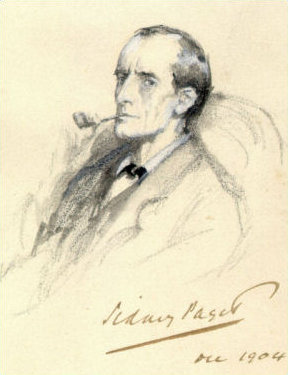
\includegraphics[width=0.3\textwidth]{pics/Sherlock_Holmes_Portrait_Paget}}
  \item and his faithful friend: John Watson
\end{itemize}
\item A fictional character, invented by Sir Arthur Conan Doyle
  \begin{itemize}
  \item in 60 stories,  published between 1887 and 1927
  \item Mainly narrated by Watson
  \end{itemize}
\item Some stories are annotated with word senses as part of our
  research in semantics
  \begin{itemize}
  \item The NTU --- Multilingual Corpus (NTU-MC)
  \item We will use and experience this during the course --- learn by doing
  \end{itemize}
\end{itemize}


\section{Revision: \\ Introduction to Semantics}

\myslide{What is Semantics}
\begin{itemize}
\item Very broadly, semantics is the study of meaning
  \begin{itemize}
  \item Word meaning
  \item Sentence meaning
  \end{itemize}
\item Layers of Linguistic Analysis
  \begin{enumerate}%\addtolength{\itemsep}{-0.75ex}
  \item Phonetics \& Phonology
  \item Morphology
  \item Syntax
  \item \emp{Semantics}
  \item Pragmatics
  \item Stylistics
  \end{enumerate}
\end{itemize}



\myslide{Meaning in the larger context}

\begin{itemize}
\item \txx{Semiotics} is the study of interpreting symbols, or \txx{signification}
  \begin{itemize}
  \item We refer to the \txx{signified}
  \item Using a \txx{signifier}\hfill Saussure
  \end{itemize}
% \item Problems with defining meaning
%   \begin{itemize}
%   \item The \txx{grounding} problem and \txx{circularity}
%   \item The boundaries of meaning: \txx{linguistic} vs \txx{encyclopedic knowledge}
%   \item Individual variation in meaning: \txx{idiolects}
%   \item Words can be combined to form an infinite number of expressions
%     \begin{itemize}
%     \item This building up of meaning is referred to as \txx{composition}
%     \item If the meaning of the whole can be built up from the parts then it is \txx{compositional}
%   \end{itemize}
% \end{itemize}
% \end{itemize}

% \myslide{Metalanguages and Notational Conventions}
\item We use language to talk about language, which can get messy.  So we
try to use certain words with very specific technical senses.

\begin{itemize}
\item \txx{technical term} $\leftarrow$ remember me!
\item \eng[gloss]{word} or \eng{utterance}: example of a word/expression being used
\item \lex{lexeme}: the abstraction of word in the lexicon
\item \iz{predicate}: the abstraction of the meaning in the lexicon/formal semantic system
\item \con{concept}: the meaning in a person's mind
\end{itemize}
\end{itemize}

\myslide{Utterances, Sentences and Propositions}

\begin{itemize}
\item \txx{utterance}: an actual instance of saying (or writing  or \ldots) something
\item \txx{sentence}: an abstraction, the type of what was said
  \begin{exe}
    \ex \eng{Caesar invades Gaul}
  \end{exe}
\item \txx{proposition}: a further abstraction, normally ignoring some non-literal meaning
  \begin{exe}
    \ex \iz{invade(Caesar, Gaul)}
  \end{exe}
\item \txx{interpretation}: our mental representation (linked to our
  existing knowledge)
\end{itemize}



% \section{Meaning, Thought and Reality}
% \MyLogo{}




\section{The meanings of words}
 \MyLogo{}


\myslide{Words carry different meanings: \lex{leave}}
\MyLogo{\url{https://lr.soh.ntu.edu.sg/ntumc/cgi-bin/showcorpus.cgi?sid_from=10000&sid_to=11000&clemma=leave}}
\begin{itemize} \addtolength{\itemsep}{0ex}
\item[10070] \eng{Nothing was \ul{left} save a few acres of ground , and the
  two-hundred-year-old house , which is itself crushed under a heavy
  mortgage .}
% leave (have left or have as a remainder) 
\item[10079] \eng{The money which my mother had \ul{left} was enough
  for all our wants , and there seemed to be no obstacle to our
  happiness . "}
%leave (leave or give by will after one's death;) 
\item[10085] \eng{He had no friends at all save the wandering
  gipsies , and he would give these vagabonds \ul{leave} to encamp upon
  the few acres of bramble- covered land which represent the family
  estate , and would accept in return the hospitality of their tents
  , wandering away with them sometimes for weeks on end .}
% leave (permission to do something;) 
\item[10107] \eng{She
  \ul{left} her room , therefore , and came into mine , where she sat for
  some time , chatting about her approaching wedding .}
%leave (move out of or depart from;) 
\item [10108]\eng{At
  eleven o'clock she rose to \ul{leave} me , but she paused at the door
  and looked back.}
%leave (move out of or depart from;) 
\item[10439] \eng{" The rest you will \ul{leave} in our hands
  . "}
% leave (put into the care or protection of someone;) 
\item[10449] \eng{And now , Miss Stoner , we must \ul{leave} you for if
  Dr. Roylott returned and saw us our journey would be in vain .
  }
% leave (move out of or depart from;) 
\item[10526] \eng{Then he turned down the lamp , and we were \ul{left} in darkness
  .}
% leave (act or be so as to become in a specified state;) 

\end{itemize}


How many different meanings?\task


\myslide{How can we represent the differences?}

\begin{itemize}
\item Definitions
\item Translations/paraphrases
\item Semantic Relations
\item Components
\item Vector Spaces
\end{itemize}


\myslide{Semantic Representations of Words}

\begin{itemize}\addtolength{\itemsep}{-1ex}
\item Divide meaning into
  \begin{itemize}
  \item \txx{reference}: the relation to the world/mental space
  \item \txx{sense}: the rest of the meaning
    \begin{itemize}
    \item \txx{denotation} the part that distinguishes the meaning
      from other meanings
    \item \txx{connotation}  cultural or emotional associations 
    \end{itemize}
  \end{itemize}
\item Introduce \con{concepts} \hfill (meaning as font-change)
  \begin{itemize}
  \item How can we represent concepts?
  \item How do we learn them?
    \begin{itemize}
    \item Typically children start off by \txx{underextending} or \txx{overextending} concepts
    \end{itemize}
  \end{itemize}
\item Example: \eng{That dog}
  \begin{itemize}
  \item reference --- the animal over there
  \item sense --- canine quadruped domesticated by man
  \item connotation --- faithful, friendly (or dirty)
  \end{itemize}
\end{itemize}



\myslide{Definitional Semantics}

%\MyLogo{\citet{Jackson:2002,Wilks+:1996}}

\begin{itemize}
\item Standard lexicographic approach to lexical semantics:
  \begin{quote}
    \textbf{semantics} = \eng{the \textcolor{blue}{study} of \textcolor{brown}{language meaning}}\\
    \textbf{tailor} = \eng{a \textcolor{blue}{person} whose \textcolor{brown}{occupation is making and altering garments}}
  \end{quote}
\item Definitions are conventionally made up of;
  \begin{itemize}
  \item \textcolor{blue}{genus}: what class the lexical item belongs to
  \item \textcolor{brown}{differentiae}: what attributes distinguish it from
  other members of that class
\end{itemize}
% \item ``Decoding'' vs.\ ``encoding'' dictionaries
\item Often hard to understand if you don't already know the meaning!
\myslide{Definitional Semantics: pros and cons}
\item Pros:
  \begin{itemize}
  \item familiarity (we are taught to use dictionaries)
  \end{itemize}
\item Cons:
  \begin{itemize}
  \item subjectivity in sense granularity (splitters vs.\ lumpers) and
    definition specificity
  \item circularity in definitions
  \item consistency, reproducibility, \ldots
  \item often focus on diachronic (historical) rather than synchronic (current) semantics 
  \end{itemize}
\end{itemize}

\myslide{Entries for \lex{leave}}
\MyLogo{\url{https://lr.soh.ntu.edu.sg/ntumc/cgi-bin/cgi-bin/wn-gridx.cgi?gridmode=ntumc-noedit&lang=eng&lemma=leave}}
\begin{description}
%  00613683-v (63)
% V2 	leave 	     	go and leave behind, either intentionally or by neglect or forgetfulness
\item [02015598-v] (72)
V1, V2 	\lex{get out, go out, leave, exit} ``move out of or depart from''
% 01494310-v (328)
% V2 	put, place, set, lay, position, pose, leave 	     	put into a certain place or abstract location
\item [02356230-v] (8)
V3 	\lex{leave, entrust} ``put into the care or protection of someone''
% 00053097-n (2)
% 	parting, farewell, leave, leave-taking 	     	the act of departing politely
      \item [02009433-v] (149)
V1 	\lex{leave, go away, go forth} ``go away from a place''
% 15139130-n (3)
% 	leave, leave of absence 	     	the period of time during which you are absent from work or duty
\item[02229055-v] (7)
V3 	\lex{leave, will, bequeath} ``leave or give by will after one's death''
% 02383440-v (14)
% V1, V2 	leave, depart, pull up stakes 	     	remove oneself from an association with or participation in
% 00360092-v (5)
% V2 	leave, leave behind 	     	be survived by after one's death
% 02721438-v (30)
% V2 	leave, allow for, allow, provide 	     	make a possibility or provide opportunity for; permit to be attainable or cause to remain
% 00136991-v (27)
% V2 	leave, leave alone, leave behind 	     	leave unchanged or undisturbed or refrain from taking
\item [02729414-v] (56) V2 	\lex{leave} ``act or be so as to become in a specified state''
\item [02730135-v] (5) V2 \lex{leave} ``have left or have as a remainder''

% 02635659-v (89)
% V2 	result, lead, leave 	     	have as a result or residue
% 02296153-v (27)
% V2, V3 	give, impart, leave, pass on 	     	transmit (knowledge or skills)
% 00613018-v (3)
% V2
\item [06690114-n] (1) \lex{leave} ``permission to do something''

\end{description}

Not to be confused with \eng{\ul{left} hand} and \eng{the \ul{leaves} fell}, \ldots .

\myslide{Paraphrases and translation}

\begin{itemize}
\item Saying the same thing in different words
  \begin{itemize}
  \item Same language = \txx{paraphrase}
  \item Different language = \txx{translation}
  \end{itemize}
\item We showed some paraphrases in the entries given above
\item If you speak another language, then you can use that to
  disambiguate may things.
  \begin{itemize}
  \item \lex{leave, entrust} = 預ける \jpn{azukeru}
  \item \lex{get out, go out, leave, exit} = 去る \jpn{saru}
  \item \lex{leave, will, bequeath} = 遺す \jpn{nokosu}
  \end{itemize}
\item Can you explain the ambiguity in \eng{The money which my mother
    had \ul{left} was enough for all our wants}?\task
\end{itemize}

\myslide{Paraphrase cues}

\begin{itemize}
\item \lex{that is to say}
  \begin{itemize}
  \item  \eng{I met him that night, and he called next day to ask if we had got home all safe, and after that we met him - that is to say, Mr Holmes, I met him twice for walks, \ldots} IDEN
  \item \eng{In three days, that is to say on Monday next  \ldots} FINA
  \end{itemize}
\item \lex{in other words}
  \begin{itemize}
  \item \eng{\ldots there is a possibility that these initials are those of the second person who was present - in other words, of the murderer. \ldots} BLAC
  \item \eng{\ldots when they closed their League offices that was a sign that they cared no longer about Mr. Jabez Wilson's presence; in other words, that they had completed their tunnel.} REDH
  \end{itemize}
\end{itemize}


\myslide{Lexical Semantics}

\MyLogo{}

\begin{itemize}
\item Lexical semantics is concerned with the identification and
  representation of the semantics of lexical items
\item If we are to identify the semantics of lexical items, we have to
  be prepared for the eventuality of a given word having 
  multiple interpretations
  \begin{itemize}
  \item \txx{Polysemy}: having multiple meanings
  \item \txx{Monosemy}: having only one meaning
  \end{itemize}
\item \txx{Homonyms} are words with two unrelated meanings:
  \begin{itemize}
  \item \txx{homographs}: same spelling 
    \\ \eng{bow} vs \eng{bow}; \eng{keep} vs \eng{keep}
  \item \txx{homophones}: same pronunciation
     \\ \eng{right} vs \eng{write}; \eng{keep} vs \eng{keep}
  \end{itemize}

\end{itemize}






% \myslide{Polysemy}

% \MyLogo{\citet{Cruse:1986,Hirst:1987,_Ravin:Leacock:2000,Pustejovsky:1995}}

% \begin{itemize}
% \item \textbf{Polysemy} = the condition of a single lexical item having
%   multiple meanings
% \item Polysemy vs.\ homonymy (cf.\ \eng{bank} vs.\ \eng{bass})
% \item Polysemy vs.\ indeterminacy (cf.\ \eng{father} vs.\ \eng{uncle})
% \item Regular/logical vs.\ irregular polysemy (cf.\ \eng{ash})
% \item Regular vs.\ complementary polysemy (cf.\ \eng{door} vs.\ \eng{farm})
% \end{itemize}




\myslide{Distinguishing Polysemes}

%The polysemy of a word can be tested by a variety of means, including:
\begin{itemize}
\item \txx{Antagonism}: can the word be used in a sentence with
  multiple \underline{competing} interpretations that are incompatible? \\[1ex]
  \eng{Kim can't  bear children}
  \begin{itemize}
  \item Cannot have children
  \item Doesn't like children
  \end{itemize}
\item \txx{Zeugma}: can the word be used in a context where multiple
  \underline{competing} interpretations are simultaneously evoked? \\[1ex]
  \eng{Kim and her visa expired}
    \begin{itemize}
    \item died
    \item ran out
    \end{itemize}
 \eng{Hitmen were quite expensive, so she decided to take out a loan and her husband.} \task
  \item  \txx{Paraphrase/Translation}: Is there more than one (clearly different) way to paraphrase/translate the word.
  \end{itemize}

\myslide{Necessary and Sufficient Conditions}

\begin{itemize}
\item Can we define words in terms of \txx{conditions}?
  \begin{itemize}
  \item \lex{zebra}
    \begin{itemize}
    \item quadruped
    \item animal \com{redundant}
    \item black and white striped
    \item herbivore
    \end{itemize}
  \end{itemize}
\item These are \txx{intrinsic}, \txx{generic} properties
\item Can we use words even if we don't know their properties?
  \begin{itemize}
  \item \lex{Kway Teow}
  \end{itemize}
\item We seem to be ok with fairly vague definitions
  \begin{itemize}
  \item What is a \lex{dog-cart}? \task
  \item What is a \lex{swamp adder}? \task
  \end{itemize}
\end{itemize}



\myslide{Words/Concepts are related in many ways}

We can also look at words (or more properly senses) in terms of their
relations to other words.

\begin{itemize}
\item \txx{Hyponymy/Hypernymy}
\item \txx{Synonymy}
\item \txx{Antonymy} (Opposites)
\item \txx{Meronymy}
    \begin{itemize}
    \item \txx{Member-Collection}
    \item \txx{Portion-Mass}
    \item \txx{Element-Substance}
    \end{itemize}
  \item \txx{Domain} (lexical field)
\end{itemize}





\myslide{Hypernymy and Hyponymy}

\begin{itemize}
\item \txx{Hyponymy}: X is a hyponym of Y iff
  $f(X)$ entails $f(Y)$ but $f(Y)$ does not entail $f(X)$ (for all or most $f$):
  \begin{quote}
    \eng{Kim has a pet \underline{dog} $\vDash$  Kim has a pet \underline{animal}}\\
    \eng{Kim has a pet \underline{animal} $\not\vDash$  Kim has a pet \underline{dog}}
  \end{quote}
  N.B.\ complications with universal quantifiers and negation:
  \begin{quote}
    \eng{Kim likes all \underline{animals} $\vDash$  Kim likes all \underline{dogs}}\\
    \eng{Kim likes all \underline{dogs} $\not\vDash$  Kim likes all \underline{animals}}
  \end{quote}
\item \txx{Hypernymy}: Y is a hypernym of X iff X is a hyponym of Y
\item Can a word have multiple hypernyms?
  \begin{exe}
    \ex \lex{tank$_1$} $\subset$ \lex{military\_vehicle$_1$}; $\subset$ \lex{tracked\_vehicle}$_1$; 
    $\subset$ \lex{armored\_vehicle$_1$}; ? $\subset$ \lex{weapon$_1$}
  \end{exe}
\end{itemize}


\myslide{What is \txx{entailment}}
\begin{quote}
  \txx{Entailment} ($\vDash$): A sentence $p$ entails a sentence $q$ when the
  truth of the first ($p$) guarantees the truth of the second ($q$),
  and the falsity of the second ($q$) guarantees the falsity of the
  first ($p$).
\end{quote}

\myslide{Properties of hypernymy/hyponymy}
  \begin{itemize}\addtolength{\itemsep}{-1ex}
  \item Asymmetric; applies at the sense level
  \item applies only to lexical items of the same word class
  \item Transitive: \lex{dog$_1$} $\subset$ \lex{mammal$_1$} $\subset$ \lex{animal$_1$}
  \item Not all nodes are lexicalized; can be multiple \\[2ex]
    \begin{tabular}{llll}
      neutral (Hyper) & male & female & child \\ \hline
%      pig & hog & sow & piglet\\
      \lex{sheep} & \lex{ram} & \lex{ewe} & \lex{lamb}\\
      \lex{cow} & \lex{bull} & \lex{\ul{cow}} & \lex{calf} \\
      \lex{goose} & \lex{gander} & \lex{\ul{goose}} & \lex{gosling}  \\
      \lex{horse} & \lex{stallion} & \lex{mare} & \lex{foal:colt/filly} \\
      \lex{dog} &  \lex{\ul{dog}} &  \lex{bitch} &\lex{puppy} \\
      \lex{snake} & \lex{\ul{snake}}& \lex{\ul{snake}}& \lex{\ul{snake}}\\
    \end{tabular}
  \item Can you do this for \lex{pig}, \lex{cat} or \lex{chicken}?\task
  \item Can you give an example of this in another language?\task
  \end{itemize}

\myslide{Language Change}

\begin{itemize}\addtolength{\itemsep}{-1ex}
\item The meanings of words change over time
\item \lex{guitar} --- ``a stringed instrument usually having six
  strings'': originally these were all made of wood
\item We then get \lex{electric guitar} --- ``a guitar with a built-in
  pickup or pickups which convert string vibrations into electrical
  signals for amplification''
\item To refer to non-electric guitars we get a new coining
  \lex{acoustic guitar} -- ``a guitar that does not require electrical
  amplification'': which used to just be guitar
  \begin{itemize}
  \item \lex{guitar} is now a hypernym of them both and can refer to
    either
  % \item we can also refer to the prototypical guitar (acoustic) using
  %   reduplication
  %   \\ \eng{What kind of guitar do you play?}  \eng{Guitar guitar}
  \end{itemize}
\newpage
  
\item Sometimes this practice becomes politically charged, although
  linguistically it is unremarkable
  \begin{itemize}
  \item \lex{woman} ``an adult female person''
  \item \lex{trans woman} ``a person who identifies as a woman but was assigned male at birth''
  \item \lex{cis woman}  ``a person who identifies as a woman and was assigned female at birth''
  \end{itemize}
  \item Can you give other examples of this in English or other languages?\task  
  
\end{itemize}
%mother, surrogate mother, stepmother, foster mother, god mother,
%adoptive mother, biological mother

% rice, cooked rice, chocolate rice, wild rice, brown rice
% 

\myslide{Synonymy}

\begin{itemize}
\item \txx{Propositional synonymy}: X is a propositional synonym of Y if
  \begin{itemize}
  \item   (i) X and Y are syntactically identical,
  \item (ii) substitution of Y  for X in a declarative sentence doesn't change its truth conditions
  \end{itemize}
  e.g., \lex{violin} and \lex{fiddle}
\item Why propositional synonymy is over-restrictive:
  \begin{itemize}
  \item syntactic identity (cf.\ \lex{eat} and \lex{devour})
  \item collocations (cf.\ \lex{cemetery} and \lex{graveyard})
  \item gradability (cf.\ \lex{sofa}/\lex{settee} vs.\ \lex{boundary/frontier})
  \end{itemize}
\end{itemize}

\myslide{Near Synonymy}
\begin{itemize}
\item Synonyms are substitutable in \textbf{some/most} rather than \textbf{all} contexts
\item Synonymy via semantics: synonyms share ``common traits'' or
  attributional overlap, walking the fine line between ``necessary
  resemblances'' and ``permissible differences'':
  \begin{quote}
      \lex{grain} vs. \lex{granule};  \lex{green} vs.\ \lex{purple}; \lex{alsation} vs. \lex{spaniel}
  \end{quote}
\item Permissible differentiation via \textbf{clarification}:
  \begin{quote}
    \eng{Here is a \underline{grain}, or \underline{granule}, of the substance.}\\
    \eng{* The cover is \underline{green}, \{or, that is to say\} \underline{purple}.}
  \end{quote}
  and \textbf{contrast}:
  \begin{quote}
    \eng{Here is a \underline{grain} or, more exactly, \underline{granule}}\\
    \eng{* He likes alsations, or more exactly, \underline{spaniels}}
  \end{quote}
\end{itemize}

\myslide{Properties of synonymy}

  \begin{itemize}
  \item Symmetric
  \item traditionally applies only to lexical items of the same word class
    \\ but pairs like \lex{can} vs \lex{be able to} suggest otherwise
  \item applied at the sense level?
  \item $\approx$ converse of polysemy
  \end{itemize}



\myslide{Antonymy (opposites)}

%\MyLogo{\citet{Cruse:1986,Miller:1990}}

\begin{itemize}
\item \txx{Simple antonyms}: the negative of one implies the positive of the other.
  \begin{exe}
    \ex \eng{dead/alive}
    \ex \eng{pass/fail}
  \end{exe}
\item \txx{Gradable Antonyms}: points  along a scale
  \begin{exe}
    \ex \eng{boiling/hot/warm/tepid/cool/cold/freezing}
    \ex \eng{like this class/fascinating/interesting/dull/boring}
  \end{exe}
\item \txx{Reverses}: reverse the direction of a motion
  \begin{exe}
    \ex \eng{ascend/descend}
    \ex \eng{up/down; right/left}
  \end{exe}
\newpage
\item \txx{Converses}: the same act from different points of view
  \begin{exe}
    \ex \eng{above/below; right/left}
    \ex \eng{employer/employee}
  \end{exe}
  (Slightly non-standard usage)
\item \txx{Taxonomic Sisters}: children of the same (grand)parent
  \begin{exe}
    \ex \eng{Monday/Tuesday/\ldots{}/Sunday}
    \\ \textnormal{in WordNet:} \lex{day of the week} $\supset$ \lex{weekday}, \lex{weekend}
    \ex \eng{LMS/English/Chinese/\ldots}
    \\  \textnormal{Context dependent}
  \end{exe}
\end{itemize}

\myslide{Meronymy}

\begin{itemize}
\item \txx{Meronomy} refers to the part-whole relation
  \begin{itemize}
  \item \txx{meronym} is the part
  \item \txx{holonym} is the whole
  \end{itemize}
  \begin{tree}
    \br{\lex{car}}{
      \br{\lex{wheel}}{\lf{\lex{tire}} \lf{\lex{rim}}}
      \br{\lex{engine}}{\br{\lex{piston}}{} \br{\lex{valve}}{}}
      \br{\lex{door}}{}
      \br{\lex{steering wheel}}{}}
  \end{tree}
\item It is not always transitive
  \begin{tree}
      \br{\lex{shirt}}{
        \br{\lex{button}}{\br{\lex{button hole}}{}}}
   \end{tree} \\
  But we don't normally say that a \lex{button hole} is part of a \lex{shirt}.
\end{itemize}

\myslide{Member-Collection}

\begin{itemize}
\item The relation between a collection and one of the units that makes it up
  \begin{exe}
    \ex \eng{tree--forest}
    \ex \eng{sheep--flock}
    \ex \eng{fish--school}
    \ex \eng{book--library}
    \ex \eng{member--band}
    \ex \eng{musician--orchestra}
    \ex \eng{student--class}
  \end{exe}
\end{itemize}

\myslide{Portion-Mass}

\begin{itemize}
\item The relation between a mass noun and a typical unit of measurement
  \begin{exe}
    \ex \eng{drop--liquid}
    \ex \eng{grain--sand/salt/truth}
    \ex \eng{sheet/ream--paper}
    \ex \eng{lump--coal (or just about anything)}
    \ex \eng{strand--hair}
    \ex \eng{rasher--bacon}
  \end{exe}
\item Similar to classifiers in many ways, e.g. in Malay
  \begin{exe}
    \ex \eng[tail]{ekor}--\eng{animal}
    \ex \eng[human]{orang}--\eng{person}
  \end{exe}
\end{itemize}

\myslide{Domain (lexical field)}
\MyLogo{Examples from WordNet 3.0}
The domain in which a word is typically used with this meaning.

\begin{exe}
  \ex \lex{driver$_1$} --- the operator of a motor vehicle
  \ex \lex{driver$_2$} --- someone who drives animals that pull a vehicle
  \ex \lex{driver$_3$} --- a golfer who hits the golf ball with a driver [\con{golf}] 
  \ex \lex{driver$_4$} --- ($\simeq$ device driver) a program that determines how a computer will communicate with a peripheral device [\con{computer science}] 
  \ex \lex{driver$_5$} --- ($\simeq$ number one wood) a golf club (a wood) with a near vertical face that is used for hitting long shots from the tee [\con{golf}] 
\end{exe}

Some \con{golf} terms: \lex{approach$_9$}, \lex{approach shot$_1$}, \lex{golf course$_1$}, \lex{links course$_1$}, \lex{wedge$_5$}, \lex{tee$_1$}, \lex{scratch$_9$}, \lex{putt$_1$}, \lex{slice$_1$}, \lex{hook$_1$}

       % TOPIC TERM->(adj) dormie#1, dormy#1
       % TOPIC TERM->(adj) greenside#1
       % TOPIC TERM->(noun) approach#9, approach shot#1
       % TOPIC TERM->(noun) chip#8, chip shot#1
       % TOPIC TERM->(noun) driving iron#1, one iron#1
       % TOPIC TERM->(noun) golf-club head#1, club head#1, club-head#1, clubhead#1
       % TOPIC TERM->(noun) golf course#1, links course#1
       % TOPIC TERM->(noun) golf equipment#1
       % TOPIC TERM->(noun) golf range#1, driving range#1
       % TOPIC TERM->(noun) heel#6
       % TOPIC TERM->(noun) plus fours#1
       % TOPIC TERM->(noun) toe#4
       % TOPIC TERM->(noun) wedge#5
       % TOPIC TERM->(noun) whip#4
       % TOPIC TERM->(noun) loft#3
       % TOPIC TERM->(noun) address#7
       % TOPIC TERM->(noun) scratch#9
       % TOPIC TERM->(noun) card#8, scorecard#1
       % TOPIC TERM->(noun) apron#2
       % TOPIC TERM->(noun) divot#2
       % TOPIC TERM->(noun) divot#1
       % TOPIC TERM->(noun) greenskeeper#1
       % TOPIC TERM->(noun) medalist#2, medallist#2, medal winner#1
       % TOPIC TERM->(noun) stroke#6
       % TOPIC TERM->(noun) birdie#1
       % TOPIC TERM->(noun) bogey#2
       % TOPIC TERM->(noun) double-bogey#1
       % TOPIC TERM->(noun) eagle#2
       % TOPIC TERM->(noun) double eagle#1
       % TOPIC TERM->(noun) par#1
       % TOPIC TERM->(verb) address#10
       % TOPIC TERM->(verb) tee off#1
       % TOPIC TERM->(verb) par#1
       % TOPIC TERM->(verb) ace#3
       % TOPIC TERM->(verb) caddie#1, caddy#1
       % TOPIC TERM->(verb) eagle#2
       % TOPIC TERM->(verb) hole up#2
       % TOPIC TERM->(verb) carry#36
       % TOPIC TERM->(verb) toe#4
       % TOPIC TERM->(verb) shank#1
       % TOPIC TERM->(verb) putt#1
       % TOPIC TERM->(verb) putt#2
       % TOPIC TERM->(verb) heel#4
       % TOPIC TERM->(verb) toe#3
       % TOPIC TERM->(verb) drive#17
       % TOPIC TERM->(verb) hole#1, hole out#1
       % TOPIC TERM->(verb) slice#2
       % TOPIC TERM->(verb) hook#4
       % TOPIC TERM->(verb) sclaff#2
       % TOPIC TERM->(verb) sclaff#1
       % TOPIC TERM->(verb) tee#1, tee up#2
       % TOPIC TERM->(verb) chip#3
       % TOPIC TERM->(verb) birdie#1
       % TOPIC TERM->(verb) eagle#1, double birdie#1
       % TOPIC TERM->(verb) double bogey#1
       % TOPIC TERM->(verb) bogey#1


\myslide{And More}
\MyLogo{}
\begin{itemize}
\item There are many, many more lexical relations advocated by various
  theories including:
  \begin{itemize}
  \item Troponymy/hypernymy (cf.\ \eng{walk} vs.\ \eng{lollop}) 
    ``way of doing something''
  \item Entailment (cf.\ \eng{snore} vs.\ \eng{sleep}) ``if you do one thing, you must be doing the other''
  \item Operator (cf.\ \eng{question} vs.\ \eng{ask})
    ``the thing you do by doing something''
  \item Magnifier (cf.\ \eng{wound} vs. \eng{badly})
    ``intensifier, diminisher''
  \item Usage (cf.\ \eng{strong-willed} vs. \eng{pig-headed} ``stubborn'')
    \\ \eng{pig-headed} is \txx{pejorative}
%  \item[] $\vdots$
  \end{itemize}
\end{itemize}


\section{Wordnet}
\MyLogo{How can we quantify these things}

\myslide{WordNet}

\MyLogo{\citet{Miller:1998:foreword,_Fellbaum:1998}}

\begin{itemize}
\item WordNet is an open-source electronic lexical database of English,
  developed at Princeton University
  \begin{quote}
    \url{http://wordnet.princeton.edu/}
  \end{quote}
\item Made up of four separate semantic nets, for each of nouns, verbs,
  adjectives and adverbs
\item WordNets exist for many languages, at LMS we work on:
  \begin{itemize}
  \item Japanese 
  \item Bahasa Malay/Indonesian
  \item Chinese
  \item The shared open multi-lingual wordnet (150+ languages) 
    \\ \url{http://compling.hss.ntu.edu.sg/omw/}
  \item Kristang
  \item Myanmar
\end{itemize}
\end{itemize}

\myslide{Wordnet Structure}
\begin{itemize}
\item Lexical items are categorised into $\sim$115K (and counting) glossed \textbf{synsets} (= synonym sets)

  \begin{quote}\smaller[2]
\begin{verbatim}
1. enrichment -- (act of making fuller or more 
   meaningful or rewarding)
2. enrichment -- (a gift that significantly increases 
   the recipient's wealth)
\end{verbatim}
  \end{quote}
\item Lexical relations at either the synset level or sense (=
  combination of lexical item and synset) level 
\item Strongly lexicalist (orginally):
  \begin{itemize}
  \item synsets only where words exist
  \item but many multiword expressions ($\approx 50\%$)
%  \item (near) absence of frame semantics
  \end{itemize}

% \newpage

% \item Other quirks/properties:
%   \begin{itemize}
%   \item 25 \textbf{unique beginners} in noun semantic net
%   \item taxonomic vs.\ functional hyponymy (cf.\ \eng{chicken} vs.\
%     \eng{bird/food})
%   \item few proper nouns and no separate classification for proper nouns
%   \end{itemize}
\end{itemize}





\myslide{Psycholinguistic Foundations of WordNet}

\MyLogo{}

\begin{itemize}
\item Strong foundation on hypo/hypernymy (lexical inheritance) based on
  \begin{itemize}
  \item   response times to sentences such as:
    \begin{quote}%\smaller
      \eng{a canary \{can sing/fly,has skin\}}\\
      \eng{a bird \{can sing/fly,has skin\}}\\
      \eng{an animal \{can sing/fly,has skin\}}
    \end{quote}
  \item analysis of anaphora:
    \begin{quote}%\smaller
      \eng{I gave Kim a novel but the \{book,?product,...\}
        bored her}\\
      \eng{Kim got a new car. It has shiny \{wheels,?wheel nuts,...\}}
    \end{quote}
  \item selectional restrictions
  \end{itemize}
\item Is now often used to calculate \txx{semantic similarity}
  \begin{itemize}
  \item The shorter the path between two synsets the more similar they are
  \item Or the shorter the path to the nearest shared hypernym, \ldots
  \end{itemize}
\end{itemize}


\myslide{Word Meaning as a Graph}
\MyLogo{}
\bigskip
\bigskip
\bigskip
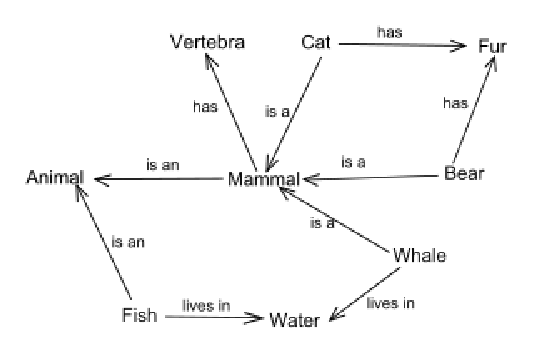
\includegraphics[height=0.75\textheight]{pics/Semantic_Net.eps}

\begin{itemize}
\item You need a very big graph to capture all meanings
\end{itemize}



\myslide{Wordnet in this course}


\begin{itemize}
\item We will use wordnet to test our skills in determining word meaning
  \begin{itemize}
  \item tag a short text from this year's story or stories
  \item discuss differences with other annotators
 \end{itemize}
\item As well as a source of examples and inspiration
\end{itemize}







\section{Where is the meaning?}





\myslide{Referential or Representational?}

One view of meaning is to define it in terms of how it constrains reality.

\begin{itemize}
\item Picture the worlds in which these sentences are true:
  \begin{exe}
    \ex \eng{I patted the dog.}
    \ex \eng{I did not pat the dog.}
  \end{exe}
\end{itemize}

Assuming that they were uttered at the same time, they are
incompatible because they cannot refer to the same
situation: the \txx{referential} view. 

But we can represent the same reality in different ways:

\begin{exe}
  \ex \eng{Ich habe Hunger} ``I have hunger''
  \ex \eng{I am hungry}
\end{exe}

\txx{Representational} theories are interested in how we represent reality,
and how our representations are influenced by conceptual structures
conventionalized in language.


 \myslide{Referential View}

 \begin{center}
   \setlength{\unitlength}{2mm}
   \begin{picture}(80,50)(0,0) \put(5,35){\oval(25,6)}
     \put(5,35){\makebox(0,0){\bf Speaker}}

     \put(25,25){\oval(25,6)}
     \put(25,25){\makebox(0,0){\bf Expression}} 

     \put(75,25){\oval(25,6)}
     \put(75,25){\makebox(0,0){\bf Referent}} 

     \put(37.5,25){\vector(1,0){25}}
     \put(50,20){\makebox(0,0){Denote}}

     \put(17.5,35){\vector(1,-0.15){45}}
     \put(50,35){\makebox(0,0){Refer}}

     \put(5,32){\vector(1,-0.20){17}}
     \put(3,30){\makebox(0,0){Say}}

   \end{picture}
 \end{center}

 The \txx{referential view} is focused on direct relationships between
 expressions (words, sentences) and things in the world (realist
 view).





 \myslide{Representational View}

 \begin{center}
   \setlength{\unitlength}{2mm}
   \begin{picture}(80,50)(0,0) \put(5,35){\oval(25,6)}
     \put(5,35){\makebox(0,0){\bf Speaker}}

     \put(25,25){\oval(25,6)}
     \put(25,25){\makebox(0,0){\bf Expression}} 

     \put(50,40){\oval(25,6)}
     \put(50,40){\makebox(0,0){\bf Concept}} 

     \put(75,25){\oval(25,6)}
     \put(75,25){\makebox(0,0){\bf Referent}} 


     % \put(37.5,25){\vector(1,0){25}}
     % \put(50,20){\makebox(0,0){Experience}}

     \put(25,28){\vector(1,0.35){26}}
     \put(30,33){\makebox(0,0){Denote}}

     \put(17.5,35){\vector(1,0.2){20}}
     \put(30,40){\makebox(0,0){Refer}}

     \put(5,32){\vector(1,-0.20){17}}
     \put(3,30){\makebox(0,0){Say}}

     \put(50,37){\vector(1,-0.35){26}}
     \put(75,33){\makebox(0,0){Represent}}
   \end{picture}
 \end{center}
\vspace{-4em} The \txx{representational view} is focused on how relationships between
 expressions (words, sentences) and things in the world are mediated by
 the mind (cognitive linguistics).  

This gives a more complex, but richer model.


\myslide{Referring vs Non-Referring}

\begin{itemize}
\item \txx{Referring expressions} are expressions that identify
  entities in the world (typically \txx{nominals})
  \begin{exe}
    \ex \eng{cat}, \jpn[that yellow bag]{ano kiiro kaban}
    \ex \eng{London Bridge}, \eng{Xiao Ming}
  \end{exe}
\item \txx{Non-referring expressions} don't have referential properties
  \begin{exe}
    \ex \eng{maybe, if, is, but}
  \end{exe}
\item Not all nominals refer
  \begin{exe}
    \ex \eng{That is \ul{an ugly dog}}
    \ex \eng{If only I had \ul{a dog}}
  \end{exe}
\item And, of course, all this is made more confusing if we model the
  fictional world and our interpretation of it as separate from the
  characters' interpretations, \ldots
\end{itemize}


\section{Deixis}


\myslide{What is Deixis}
\begin{itemize}
\item any linguistic element whose interpretation
  necessarily makes reference to properties of the
  extra-linguistic context in which it occurs is \txx{deictic}
  \begin{description}
  \item[\txx{Person}] relative to the speaker and addressee; \eng{you, me, them}
  \item[\txx{Spatial Location}] demonstratives; \eng{this, that, over there, here}
  \item[\txx{Temporal Location}] tense; \eng{yesterday, today, tomorrow}
  \item[\txx{Social Status}] relative to the social position: \eng{professor, you, uncle, boy}
  \end{description}
\item \txx{Discourse deixis}: referring to a linguistic expression or chunk of discourse
\end{itemize}

More than 90\% of the declarative sentences people utter are indexical
in that they involve implicit references to the speaker, addressee,
time and/or place of utterance in expressions like first and second
person pronouns, demonstratives, tenses, and adverbs like \lex{here}, \lex{now},
\lex{yesterday} \citep[p366]{Bar-Hillel:1954}.

\myslide{Spatial Deixis}

\begin{itemize}
\item Two way systems (English, \ldots)
  \\[2ex] \begin{tabular}{llll}
    \txx{proximal} &\lex{this} & \lex{here} &close to the speaker\\
    \txx{distal} &\lex{that} & \lex{there} & far to the speaker 
  \end{tabular}
\item Three (four) way systems (Japanese, \ldots)
    \\[2ex] \begin{tabular}{lllll}
                    & Gloss & \con{thing}   & \con{place}  \\
\hline
      \txx{proximal}  & close to speaker & \lex{kore} ``this'' & \lex{koko} ``here''\\
      \txx{medial} &close to addressee &\lex{sore} ``that''   & \lex{soko} ``there'' \\
      \txx{distal} &far from both&\lex{are} ``\,'tother'' & \lex{asoko} ``over there''  \\ \hline
      \txx{Q} & interrogative & \lex{dore} ``what'' & \lex{doko} ``where''
  \end{tabular}
  \item Can you do English \con{time}?  \task %\marginpar{\fbox{\LARGE ?}}
  \item Can you do this in another language?\task %\marginpar{\fbox{\LARGE ?}}

 % Can decompose: \lex{here} ``this place'', \lex{there} ``that place'', \lex{where} ``what place''
 % \lex{now} ``this time'',  \lex{then} ``that time'', \lex{when} ``what time''
\end{itemize}


% \mytask{try this}

% \begin{tabular}[l]{}
%   Q & close & far & further \\
%   what & this & that & 'tother \\
%   ?    & now  & then & --- \\
%   where & ? & there & over there \\
% \end{tabular}


\myslide{More Spatial Deixis}

\begin{itemize}
\item Often lexicalized:
  \begin{itemize}
  \item \lex{go, come, foreign, home, local, indigenous, national language}
  \end{itemize}
\item Can lead to \txx{discourse}/\txx{textual deixis}
  \begin{exe}
    \ex \eng{\ul{Here} we begin explaining textual deixis}
  \end{exe}
\item Often also used for time
  \begin{exe}
    \ex \eng{\ul{This year} we are trying a new kind of assignment}
  \end{exe}
\newpage
\item Spatial expressions extend to possession in many languages
  \begin{exe}
    \ex \gll \jpn{NICT-ga} \jpn{Kyoto-ni} \jpn{aru} \\
    NICT-\textsc{nom} Kyoto-\textsc{loc} be \\
    \trans NICT is in Kyoto
    \ex \gll \jpn{watashi-ni} \jpn{musuko-ga}  \jpn{aru} \\
     I-\textsc{loc}  son-\textsc{nom} be \\
    \trans I have a son (lit. a son is in me)
   \end{exe}
\end{itemize}

\myslide{Person Deixis}

\begin{itemize}
\item Minimally a three way division
\\[2ex]  \begin{tabular}{lll}
    First Person & Speaker & \lex{I} \\
    Second Person & Addressee & \lex{you} \\
    Third Person & Other & \lex{he/she/it} \\
  \end{tabular}
\item Often combined with
  \begin{itemize}
  \item \txx{gender}: \lex{he/she/it }
  \item \txx{number}: \lex{I/we}, 
    \lex{'anta} ``you:m'', \lex{'antumaa} ``you:dual'',  \lex{'antum} ``you:m:pl''
    \\ (Arabic)
  \item \txx{inclusion}: \lex{n\'uy} ``we including you'',  \lex{n\'{\i}i} ``we excluding you'' (Zayse)
  \item \txx{honorification}: \lex{kimi} ``you:inferior'', \lex{anata} ``you:equal'',
    \\ don't use pronouns for superiors: \lex{sensei} ``teacher'', \ldots (Japanese)
  \end{itemize}
\end{itemize}

\myslide{Social Deixis}

In European languages, a two-way choice in 2nd person pronominal
reference is known as the T/V distinction, based on the French forms
for ``you''.

\begin{itemize}
\item T/V distinctions in European languages
\\[2ex]  \begin{tabular}{lll}
    & Familiar 2sg & Polite 2sg \\ \hline
    French & \lex{tu} & \lex{vous} \\
    German & \lex{du} & \lex{Sie} \\
    Spanish & \lex{t\'u} & \lex{usted}
  \end{tabular}

\item Shift from asymmetric use showing \txx{power} (superior uses \lex{du}; inferior uses \lex{vous}) to symmetric use showing \txx{solidarity} (strangers use  \lex{vous}; intimates use \lex{du}): typically the socially superior person must invite the socially
  inferior person to use the familiar form
\end{itemize}

\myslide{Social Deixis can be marked on other words}
\MyLogo{It must be marked}
\begin{exe}
  \ex \jpn{Tanaka-san-ga kudasaimashita} \hfill [addressee and subject hon.]
  \trans Tanaka gave it to me (and I honor him and you)
%  \trans
 \ex \jpn{Tanaka-san-ga kudasatta} \hfill [subject honorification]
  \trans Tanaka gave it to me (and I honor him)

 \ex \jpn{Tanaka-kun-ga kuremashita} \hfill [addressee honorification]
  \trans Tanaka gave it to me (and I honor you)

 \ex \jpn{Tanaka-kun-ga kureta} \hfill [no honorification]
  \trans Tanaka gave it to me (implies I am higher status than him)

\end{exe}

\begin{itemize}
\item Find examples where someone addresses Sherlock as \eng{Holmes}
  and compare then to examples where he is addressed as \eng{Mr
    Holmes}: what is the difference? \task
\end{itemize}


\myslide{Types of Deixis}
\MyLogo{}
(a) Gestural; (b) Symbolic: (c) Non-deictic uses (Levinson 1983:66):
\begin{exe}
\ex \begin{xlist}
\ex \eng{You, you, but not you, are dismissed}
\ex \eng{What did you say?}
\ex \eng{You can never tell what they want  nowadays}
\end{xlist}
\ex \begin{xlist} 
\ex \eng{This finger hurts}
\ex \eng{This city stinks}
\ex \eng{I met this weird guy the other day}
\end{xlist}
\ex \begin{xlist} 
\ex \eng{Push, not now, but now}
\ex \eng{Let's go now rather than tomorrow}
\ex \eng{Now, that is not what I said}
\end{xlist}
\ex \begin{xlist} 
\ex \eng{Not that one, idiot, that one}
\ex \eng{That's a beautiful view}
\ex \eng{Oh, I did this and that}
\end{xlist}
% \ex \begin{xlist}
% \ex \eng{Move it from there to there
% \ex \eng{Hello, is Harry there?
% \ex \eng{There we go
% \end{xlist}  
\end{exe}




\myslide{Non-standard usage of deixis}

\begin{exe}
  \ex \eng{You take your screwdriver, right, and screw her home}
  \ex \eng{Are we ready for our medicine now, Dr Smith? }
  \ex \eng{We now turn to a discussion of globalisation in Chapter Three}
  \ex \eng{When you're hot you're hot}
  \ex \eng{Sometimes you wonder about the quality of the political leadership}
  \ex \eng{She's a beauty all right} \textnormal{[said of a car]}
\end{exe}



% \myslide{Anaphora}
% \begin{itemize}
% \item Referring to some referent described elsewhere in the discourse
% \begin{itemize}
%   \item Nominal: \eng{it, the animal}
%   \item Temporal: \eng{then} 
%   \item Backward (cataphora): if the referent comes after.
%   \end{itemize}
% \item Anaphoric elements
%   \begin{itemize}
%   \item are semantically underspecified, thus are referentially dependent upon their
%     antecedents
%   \item play an important referent tracking role in discourse, because they encode
%     topic continuity
%   \end{itemize}
% \end{itemize}


% \myslide{Strict and Sloppy Readings}
% \MyLogo{Today's joke}
% \begin{exe}
%   \ex Wife: \eng{Jim kisses \ul{his wife} goodbye before he leaves for work every morning. Why don’t you do that?}
%   \ex Husband: \eng{I don't know \ul{her} that well.}
% \end{exe}
% \begin{itemize}
% \item \txx{Sloppy anaphora}  is the wife’s intended
%   reading, where \eng{do that} is understood as ``kiss one's wife'',
%   resolving to ``kiss your (own) wife''.
% \item \txx{Strict anaphora} is the funny reading, where \eng{do that}
%   is understood as ``kiss Jim’s wife''
% \end{itemize}


%\section{Concepts}

% \myslide{Prototypes}
% \MyLogo{How things are represented in our minds}
% \begin{itemize}
% \item Concepts are organized in groups around a \txx{prototype}
% \item These have typical members (remembered as \txx{exemplars}) 
%   \begin{itemize}
%   \item What is typical \con{furniture}?
%   \item What is a typical \con{bird}?
%   \end{itemize}
% \item prototypes have \txx{characteristic feature}s
%   \begin{itemize}
%   \item has feathers
%   \item warbles
%   \item flies
%   \item lays eggs
%   \end{itemize}
% \item This work was pioneered by Eleanor Rosch (1973, 1975) (very readable)
% \end{itemize}

% % \myslide{What is a protoypical bird?}

% % \\includegraphics[width=\textwidth]{pics/prot

% \myslide{Relations between Concepts}

% \begin{itemize}
% \item Concepts are linked in many ways
% \item Most common relationship is \txx{hypernymy}: \con{dog} is-a \con{animal}
% \item Typically subordinate terms inherit properties from superordinate terms
% \\  \eng{Birds fly} so \eng{Sparrows fly}
% \item Larger units of knowledge, such as \txx{frames} are similar
%  \end{itemize}



% \myslide{Basic Level Categories}
% \begin{itemize}
% \item Some categories (concepts) seem to be more psychologically basic than others
%   \begin{itemize}
%   \item Pictures of objects are categorized faster at the basic level
%   \item Basic level names used more often in free-naming tasks
%   \item Children learn them earlier
%   \item Basic-level names are more common in adult discourse 
%   \item Basic-level categories are common in different cultures
%   \item Basic level names tend to be short
%   \item Basic-level names tend to be common in compound nouns
%   \end{itemize}
% \item
%   \begin{tabular}[t]{lll}
% superordinate & basic & subordinate \\  \hline
% \lex{vehicle} & \lex{bus} & \lex{school bus} \\
% \lex{jewelry} & \lex{necklace} & \lex{pearl necklace} \\
% \lex{animal} & \lex{dog} & \lex{poodle} 
% \end{tabular}
% \end{itemize}

% \myslide{}
% \begin{itemize}
% \item Basic level categories are a decomposition of the world into
%   maximally informative categories. 
%   \begin{itemize}
%   \item BLCs maximize the number of attributes shared by members of
%     the category
%   \item BLCs minimize the number of attributes shared with
%     other categories
%   \end{itemize}
% \item It can be hard to agree on what is the Basic Level: whereas dog
%   as a basic category is a species, bird or fish are at a higher
%   level, etc.
% \item Similarly, the notion of frequency is very closely tied
%   to the basic level, but not exactly the same.
% \end{itemize}

% \myslide{Linguistic Relativity}

% \begin{itemize}
% \item The language we think in makes some concepts easy to express,
%   and some concepts hard
% \item The idea behind \txx{linguistic relativity} is that this will
%   effect how you think
%   \begin{itemize}
%   \item Korean lexicalizes politeness and has rigid social hierarchies
%   \item English and Chinese speakers differ as to whether they
%     concepualize things as substances or individuals
%   \item Gendered language speakers have different connotations: \lex{key}
%     \begin{itemize}
%     \item (German: masculine) `hard, heavy, jagged, metal, and useful'
%     \item (Spanish: feminine)  `golden, intricate, little, lovely, shiny, and tiny'
%     \end{itemize}
%   \item It is easier to differentiate colors that you have names for
%   \end{itemize}
% \item Most confirmed differences are very, very subtle
% \end{itemize}


% \myslide{The Sapir-Whorf Hypothesis}

% \begin{description}
% \item[strong]  language determines thought and that linguistic categories limit and determine cognitive categories
% \item[weak]  linguistic categories and usage influence thought and certain kinds of non-linguistic behaviour
% \end{description}

% The terms "Strong/Weak Sapir-Whorf Hypothesis" is widely used even though Edward
% Sapir and Benjamin Lee Whorf never co-authored anything and never
% stated their ideas in terms of a hypothesis let alone with two versions.

% \myslide{What Whorf actually said}
% \begin{quotation}
%   We dissect nature along lines laid down by our native language. The
%   categories and types that we isolate from the world of phenomena we
%   do not find there because they stare every observer in the face; on
%   the contrary, the world is presented in a kaleidoscope flux of
%   impressions which has to be organized by our minds—and this means
%   largely by the linguistic systems of our minds. We cut nature up,
%   organize it into concepts, and ascribe significances as we do,
%   largely because we are parties to an agreement to organize it in
%   this way—an agreement that holds throughout our speech community and
%   is codified in the patterns of our language [\ldots] all observers
%   are not led by the same physical evidence to the same picture of the
%   universe, unless their linguistic backgrounds are similar, or can in
%   some way be calibrated.
% \\ \hfill Whorf (Carroll; Ed.); 1956: pp. 212–214
% \end{quotation}


% \myslide{Language, Thought and Reality}

% \begin{itemize}\addtolength{\itemsep}{-1ex}
% \item Do we really think in language? 
%   \begin{itemize}
%   \item We can think of things we don't have words for
%   \item Language under-specifies meaning
%   \end{itemize}
% \item Maybe we store a more abstract representation
% \\ \txx{the language of thought} or \txx{Mentalese}
% \item Does the world exist outside of our minds?
% \item If so, can we truly perceive it?
% \item Many linguists side-step these issues: \txx{lexical semantics}
% \item Many simplify them: \txx{formal semantics}
% \item Some meet them head on: \txx{conceptual/cognitive semantics}
% \end{itemize}


\section{What is a word?}

\myslide{Defining \lex{word}}

\begin{itemize}
\item How many words are there in the following?
  \begin{exe}
  \ex \eng{He who laughs last laughs longest.}
  \ex \eng{If he is right and I am wrong, are we both in trouble?}
  \ex \eng{I'm gonna go to the  station-master.}
  \ex \eng{Sorry to knock you up, Mr Holmes.}
  \ex \eng{他们结婚了} \eng{ta1men jie2hun1 le} ``they got married'' (\eng{他们结了婚})
\end{exe}  

\item \txx{Tokens}: Individual instances of a class
\item \txx{Types}: The class as a whole
\end{itemize}
\newpage
\begin{itemize}
\item  Why do we need a definition for \lex{word}?
  \begin{itemize}
  \item Psychological reality:  People can divide language into words
  \item Phonological contours:  People pronounce words as unit
  \item Orthographic practice: Many languages put spaces between words
(although this practice only began around 600 CE for Latin, and did
not spread to all European languages 'til as late as the 1600s)
 \begin{itemize}
 \item Some put them between phrases (Korean)
 \item Some words include spaces \eng{New York}, \eng{ad hoc}
  \end{itemize}
\end{itemize}
\end{itemize}

\myslide{Bloomfield's grammatical definition}

\begin{quote}
A word, then, is a free form, which does not consist
entirely of (two or more) lesser free forms; in brief, a
word is a \textit{minimum free form}.
\begin{flushright}
  (Bloomfield 1984: p178) 
\end{flushright}
 \end{quote}

In practice, the definition is somewhat task specific: it may make more sense to talk of \txx{orthographic words}, \txx{semantic words} or \txx{predicates}, \ldots .

% \section{Derivational Relations}

% \myslide{Diathesis Alternations}

% \MyLogo{\citet{Levin:1993}}

% \begin{itemize}
% \item \txx{Causative/inchoative alternation}:
%   \begin{quote}
%     \eng{Kim \ul{broke} the window} $\leftrightarrow$ \eng{The window \ul{broke}}
%     \\ also \eng{the window \ul{is broken}} (state)
%   \end{quote}
% \item \txx{Middle construction alternation}:
%   \begin{quote}
%     \eng{Kim \ul{cut} the bread} $\leftrightarrow$ \eng{The bread \ul{cut} easily}
%   \end{quote}
% \item \txx{Conative alternation}:
%   \begin{quote}
%     \eng{Kim \ul{hit} the door} $\leftrightarrow$ \eng{Kim \ul{hit} at the door}
%   \end{quote}
% \item \txx{Body-part possessor ascension alternation}:
%   \begin{quote}
%     \eng{Kim \ul{cut} Sandy's arm} $\leftrightarrow$ \eng{Kim \ul{cut} Sandy on the arm}
%   \end{quote}
% \end{itemize}




% \myslide{Diathesis Alternations and Verb Classes}

% \MyLogo{\citet{Levin:1993}}

% \begin{itemize}
% \item A verb's (in)compatibility with different alternations is a strong
%   predictor of its lexical semantics:
%   \begin{quote}\smaller[1]
%     \begin{tabular}{ccccc}
%       & \lex{break} & \lex{cut} & \lex{hit} & \lex{touch} \\
%       Causative & YES & NO & NO & NO \\
%       Middle & YES & YES & NO & NO \\
%       Conative & NO & YES & YES & NO \\
%       Body-part & NO & YES & YES & YES \\
%     \end{tabular}
%     \vspace{3ex}

%     \larger[1]
%     \lex{break} = \{\eng{break, chip, crack, crash, crush, ...}\}\\
%     \lex{cut} = \{\eng{chip, clip, cut, hack, hew, saw, ...}\}\\
%     \lex{hit} = \{\eng{bang, bash, batter, beat, bump, ...}\}\\
%     \lex{touch} = \{\eng{caress, graze, kiss, lick, nudge, ...}\}
%   \end{quote}

% %\newpage


% \item \textbf{Corollary}: we can predict the syntax of novel words we
%   are given the semantic class for

% \item The principal weakness of syntax-based verb classification is that
%   there are often subtle divergences in semantics between synonyms (cf.\
%   \lex{eat} vs.\ \lex{devour} vs.\ \lex{gobble})
% \end{itemize}

% \myslide{Agentitive Nouns}
% \MyLogo{}
% \begin{itemize}
% \item The entity who/which performs the action of the verb
%   \\ \textbf{verb} + \lex{-er, -or, -ant}
%   \begin{exe}
%     \ex \lex{murderer, commentator, whaler, director, computer}
%     \ex ?? \lex{undertaker, cooker, footballer, crofter}
%   \end{exe}
% \item Should \lex{murderer} be listed separately from \lex{murder} in
% the dictionary? Why or why not?\task
% \item Also the undergoer: \textbf{verb} + \lex{-ee}: \lex{employee}
% \item \lex{-er\,$|$-or} has equivalents in most languages:
%   \\ Japanese: 員, 者, 人, 機, \ldots
% \end{itemize}


% \section{Lexical Universals}

% \myslide{Color Terms}

% \begin{itemize}
% \MyLogo{See also: \url{http://wals.info/chapter/133}: Colour Terms
% by Paul Kay and Luisa Maffi}
% \item \txx{Basic Color Terms}
%   \begin{itemize}
%   \item Monolexemic
%   \item Not a hyponym of any other color
%   \item Can be widely applied
%   \item Not derived from a noun
%   \end{itemize}
% \item Seem to come in an order
% \hspace*{-4em}\[ \left\{ \begin{array}[c]{l}
%     \mbox{\con{white/dark}} \\  \mbox{\con{black/light}}
%   \end{array} \right\}
%    < \mbox{\con{red}} < 
%  \left\{ \begin{array}[c]{l}
%     \mbox{\con{green}} \\  \mbox{\con{yellow}}
%   \end{array} \right\}
%  < \mbox{\con{blue}} < \mbox{\con{brown}} <  
% \left\{ \begin{array}[c]{l}
%     \mbox{\con{purple}} \\  \mbox{\con{pink}} \\ \mbox{\con{orange}} \\  \mbox{\con{grey}}
%   \end{array} \right\} \]
% \item \txx{Focal Colors} are related to the neurophysiology of our visual system
% \end{itemize}

% \myslide{Core Vocabulary}
% \MyLogo{\url{en.wiktionary.org/wiki/Appendix:Swadesh_list}}
% \begin{itemize}
% \item Some universal terms can be used to compare languages
%   \begin{itemize}
%   \item lexicostatistics (quantitative language relatedness assessment)
%   \item glottochronology (language divergence dating)
% \end{itemize}
% \item The \txx{Swadesh list}, developed by Morris Swadesh from 1940 onward 
% \end{itemize}
% \vspace*{-2ex}
% I, You, we, this, that, who, what, not, all, many, one, two, big,
% long, small, woman, man, person, fish, bird, dog, louse, tree, seed,
% leaf, root, bark, skin, flesh, blood, bone, grease, egg, horn, tail,
% feather, hair, head, ear, eye, nose, mouth, tooth, tongue, claw, foot,
% knee, hand, belly, neck, breasts, heart, liver, drink, eat, bite, see,
% hear, know, sleep, die, kill, swim, fly, walk, come, lie, sit, stand,
% give, say, sun, moon, star, water, rain, stone, sand, earth, cloud,
% smoke, fire, ash(es), burn, path, mountain, red, green, yellow, white,
% black, night, hot, cold, full, new, good, round, dry, name
% \vspace*{-1ex}
% \begin{itemize}
% \item Available in many languages (hundreds) 
% \end{itemize}
% \vspace*{-1ex}

\myslide{What if we had fewer words?}

\eng{He was a fine creature, this man of the old English soil, simple, straight and gentle, with his great, earnest, blue eyes and broad, comely face. His love for his wife and his trust in her shone in his features. Holmes had listened to his story with the utmost attention, and now he sat for some time in silent thought.} DANC

\begin{itemize}
\item Can we get the same message (denotation and connotation) with a
smaller vocabulary? \url{http://xkcd.com/simplewriter/}
\item It is hard!
\item That is why we have so many words
\item and why some writers are better than others.
\end{itemize}


\myslide{Conclusions}

\begin{itemize}
\item We learned about how to talk about meaning
\end{itemize}

\myslide{Acknowledgments and References}

\begin{itemize}
\item Definitions from WordNet: \url{http://wordnet.princeton.edu/}
\item Images from
  \begin{itemize}
  \item the Open Clip Art Library: \url{http://openclipart.org/}
  \item Steven Bird, Ewan Klein, and Edward Loper (2009) 
     \textit{Natural Language Processing with Python}, O'Reilly Media
    \\ \url{www.nltk.org/book}
\end{itemize}
%\item Problems  partially based on exercises from Saeed (2003)
\item Video: Dead parrot sketch by Monty Python
\end{itemize}



\myslide{Synonyms for a \lex{dead} Parrot}

\begin{quote} \large
  \lex{be dead, be demised, be deceased, pass on, be no more, cease to be,
  expire, go to meet one's maker, be a stiff, be bereft of life,
  rest in peace, push up the daisies, one's metabolic processes are
  now history, be off the twig, kicked the bucket, shuffle off this
  mortal coil, ring down the curtain, join the choir invisible, be an
  ex-parrot}
\end{quote}

From the ``Dead Parrot Sketch'', also known as the ``Pet Shop Sketch''
or ``Parrot Sketch'', originally in \textit{Monty Python's Flying Circus},
first performed in the eighth episode of the show's first series,
"Full Frontal Nudity" (7 December 1969).









  
\small
\bibliographystyle{aclnat}
\bibliography{abb,mtg,nlp,ling}





\end{document}

%%% Local Variables: 
%%% coding: utf-8
%%% mode: latex
%%% TeX-PDF-mode: t
%%% TeX-engine: xetex
%%% End: 

